\newpage
\section{Problem 2: FREQUENCY DOMAIN}\label{problem-2-frequency-domain}
In this problem, please perform Fourier transform and observe the relation between the spatial domain and the frequency spectrum. You may adopt tools for Fourier transform. The recommended tools are listed in the Appendix.

Original image \nameref{sample2} for question \nameref{2_a} \nameref{2_b}, \nameref{2_c}.
\begin{figure}
    \centering
    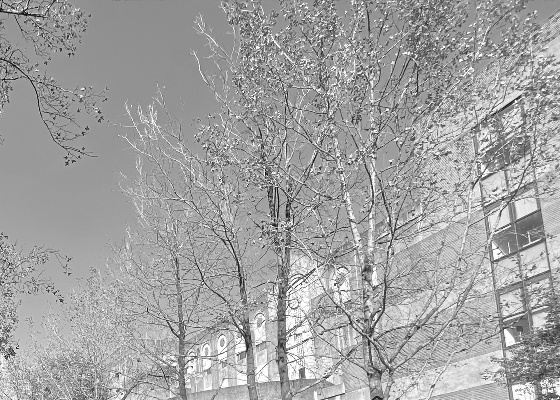
\includegraphics[width=0.7\textwidth]{src/sample2.png}
    \caption{\textbf{sample2.jpg}}
    \label{sample2}
\end{figure}

\subsection{(a)}\label{2_a}
Perform Fourier transform on \textbf{sample2.png} to obtain its frequency spectrum and output it as \textbf{result5.png}. (Please take the log magnitude of the absolute value and center the low frequency part at the origin for visualization.)

\paragraph{Motivation}
\textbf{Frequency domain} could give us other respect of images.
For visualization, \textbf{log transformation} could expand the dynamic range of low gray-level values and compress of high gray-level values.

\paragraph{Approach}
Follow the steps in \textbf{Lec 9 page 12---13}.
\begin{enumerate}
    \item Centering and Fourier transform with \\
	\[
	    \mathcal{F}[f(j, k)(-1)^{j+k}] = F(u - \frac{M}{2}, v - \frac{N}{2})
	\]
	Take use of \texttt{np.fromfunction(lambda i, j: (-1)**(i + j), shape)}.
	Than \texttt{fft2} on it.
    \item Take log and absolute value of \(F[u - \frac{M}{2}, v - \frac{N}{2}]\) to get results \(F\textnormal{\textquotesingle}(u, v)\).
    \item Normalize \(F\textnormal{\textquotesingle}(u, v)\) to \([0, 1]\) then scale to \([0, 255]\)
\end{enumerate}

\paragraph{Performance of results}
In the end, based on \nameref{sample2}.

Result of problem 2(a): \nameref{result5}.
\begin{figure}
    \centering
    \includegraphics[width=0.7\textwidth]{src/result5.png}
    \caption{\textbf{result5.jpg} Log axis of frequency domain}
    \label{result5}
\end{figure}

\paragraph{Discussion}

\subsection{(b)}\label{2_b}
Based on the result of part (a), design and apply a low-pass filter in the frequency domain and transform the result back to the pixel domain by inverse Fourier transform. The resultant image is saved as \textbf{result6.png}. Please also design a low-pass filter in the pixel domain which behaves similarly to the one you design in the frequency domain. Output the result as \textbf{result7.png} and provide some discussions.

\paragraph{Motivation}
Filtering in frequency domain is easy to implement with Fourier transform. And it just design the filter matrix \(h(j, k)\) \textbf{multiply} rather than \textbf{convolution} on frequency domain. So we could conduct the operation on overall image instead of sub-array on spatial domain.

\paragraph{Approach}
I choose \textbf{Gaussian filter}. As it is easy to specify and correspond between frequency and spatial domain.
\begin{enumerate}
    \item Design Gaussian low-pass filter.
	\[
	    H_{\mbox{low}}(u, v) = \exp \left(\frac{-D(u, v)^2}{(2D_{0}^{2})} \right)
	\]
	where \(D(u, v) = [(u - \frac{M}{2})^{2} + (v - \frac{N}{2})^{2}]^{\frac{1}{2}}\) \\
	\(D_{0}\) is cutoff, reflect standard deviation \(\sigma\) in Gaussin distribution.
    \item Conduct Fourier transform \(F(u, v)\) then mutiply \(H_{\mbox{low}}(u, v)\) to get \(G(u, v)\)
    \item Conduct inverse Fourier transform and shift (by \(-1^{j + k}\)) to get \(g_{\mbox{low}}(j, k)\).
\end{enumerate}

Correspond to frequency domain filtering, I implement spatial domain Gaussian filter.
\begin{enumerate}
    \item Design Gaussian low-pass filter.
	\[
	    h_{\mbox{low}}(j, k) = \frac{1}{2 \pi D_{0}^{2}} \exp \left(-\frac{(j - \frac{\mbox{kernel size}}{2})^{2} + (v - \frac{\mbox{kernel size}}{2})^{2}}{2 D_{0}^{2}} \right)
	\]
	where \(\mbox{kernel size}\), \\
	\(D_{0}\) is cutoff, reflect standard deviation \(\sigma\) in Gaussin distribution.
    \item Conduct convolution by filter \(g_{\mbox{low}}(j, k) = f(j, k) \ast h_{\mbox{low}}(j, k)\) 
\end{enumerate}

\paragraph{Performance of results}
In the end, I choose the settings of \(D_{0}=50\) on both frequency domain and spatial domain. And choose \(\mbox{kernel size} = 5\) on spatial domain filter size.

For Gaussian low-pass filter on frequency domain,
result of problem 2(b): \nameref{result6}.
\begin{figure}
    \centering
    \includegraphics[width=0.7\textwidth]{src/result6.png}
    \caption{\textbf{result6.jpg} Low-pass filter in frequency domain}
    \label{result6}
\end{figure}

For Gaussian high-pass filter on spatial domain,
result of problem 2(b): \nameref{result7}.
\begin{figure}
    \centering
    \includegraphics[width=0.7\textwidth]{src/result7.png}
    \caption{\textbf{result7.jpg} Low-pass filter in spatial domain}
    \label{result7}
\end{figure}

\paragraph{Discussion}
Compare \nameref{result6} with \nameref{result7}.

\nameref{result6} provide more \textbf{blurry} results although I choose the same \(D_{0}\) (\(\sigma\)) on both domain. And I find out the white line on boundary. It could be my implementation error.

\nameref{result7} could result \textbf{lattice effects} on each sub-region. I consider that it caused by the average/ convolution on each sub-array.

\subsection{(c)}\label{2_c}
Based on the result of part (a), design and apply a high-pass filter in the frequency domain and transform the result back to the pixel domain by inverse Fourier transform. The resultant image is saved as \textbf{result8.png}. Please also design a high-pass filter in the pixel domain which behaves similarly to the one you design in the frequency domain. Output the result as \textbf{result9.png} and provide some discussions.

\paragraph{Motivation}
High-pass filter is another view in frequency domain. It correspond the \textbf{edge} on image.

\paragraph{Approach}
I choose \textbf{Gaussian filter}. And we could treat the high-pass filter as \textbf{original image minus low-pass filter}.
For frequency domain,
\begin{enumerate}
     \item Design Gaussian high-pass filter.
	\[
	    H_{\mbox{high}}(u, v) = 1 - H_{\mbox{low}}(u, v)
	\]
    \item And follow process of frequency domain in \ref{2_b}.
\end{enumerate}

Slightly different with frequency domain
\begin{enumerate}
    \item Conduct spatial domain Gaussian low-pass filter in \ref{2_b}.
    \item Original image minus low-pass result.
	\[
	    g_{\mbox{high}}(j, k) = f(j, k) - g_{\mbox{low}}(j, k)
	\]
\end{enumerate}
As I find out that we couldn't change kernel filter before convolution.

\paragraph{Performance of results}
In the end, I choose the same settings as \ref{2_b}.

Result of problem 2(c): \nameref{result8}.
\begin{figure}
    \centering
    \includegraphics[width=0.7\textwidth]{src/result8.png}
    \caption{\textbf{result8.jpg} High-pass filter in frequency domain}
    \label{result8}
\end{figure}

Result of problem 2(c): \nameref{result9}.
\begin{figure}
    \centering
    \includegraphics[width=0.7\textwidth]{src/result9.png}
    \caption{\textbf{result9.jpg} High-pass filter in spatial domain}
    \label{result9}
\end{figure}

\paragraph{Discussion}
Compare \nameref{result8} with \nameref{result9}.

\nameref{result8} gives \textbf{thicker} and \textbf{fill} edges of image.

\nameref{result9} give \textbf{fragile} on the \textbf{large black region}.

Original image \nameref{sample3} for question \nameref{2_d} \nameref{2_e}.
\begin{figure}
    \centering
    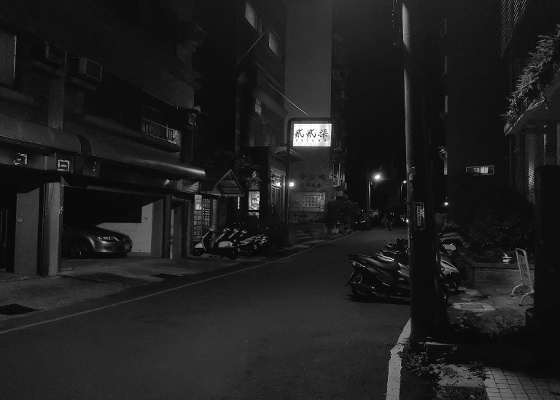
\includegraphics[width=0.7\textwidth]{src/sample3.png}
    \caption{\textbf{sample3.jpg}}
    \label{sample3}
\end{figure}

\subsection{(d)}\label{2_d}
Perform Fourier Transform on \textbf{sample3.png} and output it as \textbf{result10.png}. Please discuss what you observe in \textbf{sample3.png} and \textbf{result10.png}.

\paragraph{Motivation}
It is relative simple conduct periodic noise reduction on frequency domain.

\paragraph{Approach}
The same steps as \ref{2_a}

\paragraph{Performance of results}
In the end, based on \nameref{sample3}.

Result of problem 2(d): \nameref{result10}.
\begin{figure}
    \centering
    \includegraphics[width=0.7\textwidth]{src/result10.png}
    \caption{\textbf{result10.jpg} Fourier Transform on \nameref{sample3}}
    \label{result10}
\end{figure}

\paragraph{Discussion}
Observe in \nameref{sample3} and \nameref{result10}.
Here we could see the \textbf{vertical ripple} on the original image is corresponding to \textbf{two bright spots on horizontal center line}.

\subsection{(e)}\label{2_e}
Try to remove the undesired pattern on \textbf{sample3.png} and output it as \textbf{result11.png}.

\paragraph{Motivation}
It is relative simple conduct periodic noise reduction on frequency domain.

\paragraph{Approach}
Follow the steps in \textbf{Lec 9 page 35}.
\begin{enumerate}
    \item Use \textbf{butterworth} on two bright spots on horizontal center line on frequency domain.
    \item Conduct inverse Fourier transform to recover original image.
\end{enumerate}

\paragraph{Performance of results}
In the end, I choose the butterworth range with
\begin{itemize}
    \item \texttt{M//2 - 1: M//2 + 2, 165:185}
    \item \texttt{M//2 - 1: M//2 + 2, 455:475}
\end{itemize}
where \texttt{M} is center horizontal line.

Result of problem 2(e): \nameref{result11}.
\begin{figure}
    \centering
    \includegraphics[width=0.7\textwidth]{src/result11.png}
    \caption{\textbf{result11.jpg} Noise cleaning of \nameref{sample3}}
    \label{result11}
\end{figure}

\paragraph{Discussion}
Get critical removal points is crucial for denoising in frequency domain.
Maybe we could develop \textbf{automatic process} to denoise ripple noise image in future.

